\documentclass[a4paper,14pt]{article}
\usepackage{extsizes}
\usepackage{amsmath}
\usepackage{amssymb}
\everymath{\displaystyle}
\usepackage{geometry}
\usepackage{fancyhdr}
\usepackage{multicol}
\usepackage{graphicx}
\usepackage[brazil]{babel}
\usepackage[shortlabels]{enumitem}
\usepackage{cancel}
\columnsep=2cm
\hoffset=0cm
\textwidth=8cm
\setlength{\columnseprule}{.1pt}
\setlength{\columnsep}{2cm}
\renewcommand{\headrulewidth}{0pt}
\geometry{top=1in, bottom=1in, left=0.7in, right=0.5in}

\pagestyle{fancy}
\fancyhf{}
\fancyfoot[C]{\thepage}

\begin{document}
	
	\noindent\textbf{8FMA30~-~Matemática} 
	
	\begin{center}Quadriláteros em figuras 3-D (Versão estudante)
	\end{center}
	
	
	\noindent\textbf{Nome:} \underline{\hspace{10cm}}
	\noindent\textbf{Data:} \underline{\hspace{4cm}}
	
	%\section*{Questões de Matemática}
	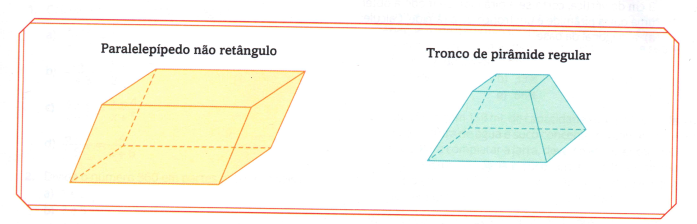
\includegraphics[width=1\linewidth]{8FMA30_imagens/aula30-1}
	\begin{multicols}{2}
		\begin{enumerate}
	    	\item Um paralelepípedo não retângulo tem duas faces retangulares 4 cm x 9 cm, duas faces quadradas de lado 4 cm e duas faces em forma de paralelogramos de base 9 cm e altura relativa a essa base com medida 2 cm, ou seja, cada paralelogramo tem área igual a 18 cm². Qual é a área total desse paralelepípedo? \\\\\\\\\\\\\\\\\\\\\\\\\\\\\\
	    	\item Uma caixa de chocolate tem a forma de um tronco de pirâmide regular\\
	    	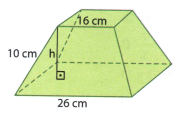
\includegraphics[width=0.9\linewidth]{8FMA30_imagens/aula30-2}
	    	\begin{enumerate}[a)]
	    		\item Identifique a forma de cada uma das faces da caixa.\\\\\\\\\\\\\\\\\\\\\\\\
	    		\item Calcule a área total da caixa.\\\\\\\\\\\\\\\\\\\\
	    		\item Calcule a altura da caixa (indicada por $h$, no desenho).\\\\\\\\\\\\\\\\\\\\
	        \end{enumerate}
            \item Considere uma pirâmide regular de base quadrada cujas arestas da base medem 12 cm e as arestas laterais medem 10 cm. Com um plano paralelo à base, há 3 cm do vértice, corta-se a pirâmide de modo a obter uma outra pirâmide e um tronco de pirâmide. Calcule:
            \begin{enumerate}[a)]
            	\item a diagonal da base.\\\\\\\\\\\\
            	\item a altura da pirâmide.\\\\\\\\\\\\\\\\\\\\
            	\item a altura da face lateral.\\\\\\\\\\\\\\\\\\\\
            	\item a área total do tronco.\\\\\\\\\\\\\\\\\\\\
            \end{enumerate}
            \textbf{Desafio olímpico}
\\\\
            Na figura, os pontos $C$ e $F$ pertencem aos lados $BD$ e $AE$ do quadrilátero $ABDE$, respectivamente. Os ângulos $\hat{B}$ e $\hat{E}$ são retos e os segmentos $AB$, $CD$, $DE$ e $FA$ tem suas medidas indicadas na figura. Qual é a área do quadrilátero $ACDF$?
            \begin{center}
            	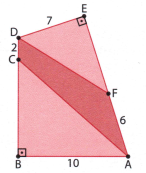
\includegraphics[width=0.7\linewidth]{8FMA30_imagens/aula30-3}
            \end{center}
            \begin{enumerate}[a)]
            	\item 16
            	\item 21
            	\item 31
            	\item 33
            	\item 40
            \end{enumerate}
            \item As faces laterais de um tronco de pirâmide regular de base quadrada são trapézios isósceles de bases 4m e 7 m e altura 6 m. Determine a área total desse tronco.\\\\\\\\\\\\\\\\\\\\
            \item Um paralelepípedo é formado por dois retângulos de dimensões 5 $\times$ 4 e 2 paralelogramos de lados 5 e 9 e altura 4, relativa ao lado de medida 9. \\\\\\\\\\\\\\\\\\\\
            \item Quais são as medidas dos lados dos outros dois retângulos que formam o paralelepípedo?\\\\\\\\\\\\\\\\\\\\
            \item Qual é a área total do paralelepípedo?\\\\\\\\\\\\\\\\\\\\
            \item Numa famosa rede de fast food chinês o yakisoba é vendido em caixas fechadas que tem o formato de tronco de pirâmide regular de base quadrada cujas arestas das bases medem 8 cm e 18 cm e a altura é 12 cm.
            \begin{enumerate}[a)]
	            \item Se a cada dia são vendidos 90 yakisobas em uma loja, qual a área mínima de papel para produzir tais embalagens?\\\\\\\\\\\\\\\\\\\\
	            \item O volume de um tronco de pirâmide regular de base quadrada é dado por:\\ $V=\frac{h}{3}(S+\sqrt{Ss}+s)$,\\ em que h é a altura do tronco, S é a área da base maior e s é a área da base menor.
	            Qual o volume máximo de yakisoba que pode ser colocado na caixa?\\\\\\\\\\\\\\\\\\\\\\
        	\end{enumerate}
        	\item Um bloco retangular de isopor de arestas 12,16 e 20 foi recortado de moda formar um paralelepípedo não retângulo, como mostra a figura:
        	\begin{center}
        		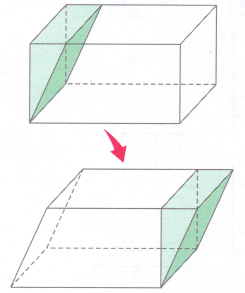
\includegraphics[width=0.7\linewidth]{8FMA30_imagens/aula30-4}
        	\end{center}
        	O que aconteceu com a área total do bloco: aumentou, diminuiu ou permaneceu a mesma?
   	    \end{enumerate}
       $~$ \\ $~$ \\ $~$ \\ $~$ \\ $~$ \\ $~$ \\ $~$ \\ $~$ \\ $~$ \\ $~$ \\ $~$ \\ $~$ \\ $~$ \\ $~$ \\ $~$ \\ $~$ \\ $~$ \\ $~$ \\  $~$ \\  $~$ \\ 
    \end{multicols}

\end{document}